\chapter{Entwicklung der Schlüsselelemente}
\section{Übersicht des gesamten Modells}

\section{Schaltplan}

\section{BMS und Laden}

\section{Mecanum}
Als besonderes Merkmal des TEGGLA fallen sofort die besonderen Räder auf. Hierbei handelt es sich um sogenannte Mecanum-Räder. 

Hierbei handelt es sich von Bengt Ilon 1972 erfundene Räder, die es dem Fahrzeug erlauben sich in drei Freiheitsgraden zu bewegen.

Dies wird ermöglicht durch die um 45\degree{} gedrehten Rollen auf den Rädern, sodass diese wie ein X aussehen.
Durch unterschiedliche Drehrichtung und Drehgeschwindigkeit der Motoren kann das Fahrzeug in jegliche Richtungen innerhalb der Ebene beweget werden. (vgl. Abb~\ref{bild:mecanum})

\begin{figure}[!ht]
	\centering
	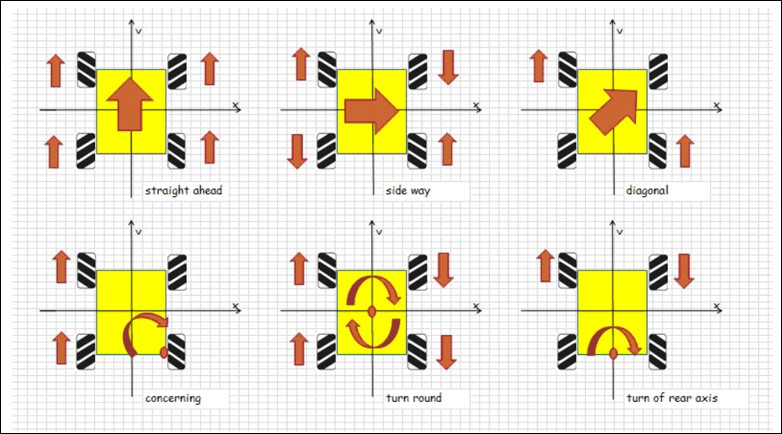
\includegraphics[width=\textwidth]{bilder/mecanum.jpg}
	\caption{Freiheitsgrade von Mecanum \cite{link:mecanum}}
	\label{bild:mecanum}
\end{figure}

Die jeweiligen zu Motorgeschwindigkeiten lassen sich hierbei durch Formeln~\ref{eq:mec1}--\ref{eq:mec2} berechnen.\\

$V_x =$ Motorgeschwindigkeit des x-ten Rads im Uhrzeigersinn (beginnend vorderes linkes Rad)\\
$V_d =$ gewünschte Roboter Geschwindigkeit $[-1, 1]$\\
$\theta_d =$ gewünschter Winkel $[0, 2\pi]$\\
$V_\theta =$ gewünschte Rotationsgeschwindigkeit $[-1, 1]$\\


\begin{align}
	V_1 = V_d\sin{(\theta_d+\frac{\pi}{4})} + V_\theta \label{eq:mec1}\\
	V_2 = V_d\cos{(\theta_d+\frac{\pi}{4})} - V_\theta\\
	V_3 = V_d\cos{(\theta_d+\frac{\pi}{4})} + V_\theta\\
	V_4 = V_d\sin{(\theta_d+\frac{\pi}{4})} - V_\theta \label{eq:mec2}
\end{align} 
\captionof{figure}{Formeln für individuellen Motoren \cite{link:mecanum}}

Bei den in diesem Praktikum verwendeten Rädern handelt es sich um eine Modifierung der Mecanum von Jonah Innoart von dem Internetportal Thingiverse \cite{link:mecanum44}.

\section{Planetengetriebe}

\section{ESP-32 vs. ESP-8266}
Bei dem vom Lehrstuhl gestellten ESP-8266 handelt es sich um ein WiFi-fähigen Microcontroller der chinesischen Firma ``espressif''.
Dieser besitzt 17 GPIO Pins, wovon jedoch lediglich 11 Pins nutzbar sind, da 6 an den externen SPI Flash angeschlossen sind.
Da dies wie in Tabelle~\ref{table:pins} aufgezeigt nicht für unsere Zwecke reicht, musste auf den leistungsstärkeren ESP-32 ausgewichen werden.

\begin{table}[!ht]
\centering
\begin{tabular}{lr}
	\multicolumn{2}{c}{Benötigte Pins} \\ 
	\midrule[3pt] 
	4x PWM & Motor Enable \\ 
	\midrule 
	8x Output & Motor Richtung \\ 
	\midrule 
	2x I$^2$C & Gyroskop \\ 
	\midrule 
	1x ADC & Batteriespannung \\ 
	\midrule
	\midrule 
	\multicolumn{2}{c}{15 Pins} \\ 
	 
\end{tabular} 
\caption{Aufzählung benötigter Pins} 
\label{table:pins}
\end{table} 

Obwohl die Anzahl der Pins das ausschlaggebenede Argument für einen Austausch des MicroControllers war, bringt dieser natürlich weitere Vorteile mit sich.

Beispielsweise profitiert die später genauer erklärte Website stark davon, auf einen zweiten Core ausgelargert werden zu können.

Siehe Tabelle~\ref{table:esp32} für einen Vergleich der beiden MicroController anhand der für dieses Projekt relevanten Faktoren.


\begin{table}[!ht]
\centering	
\begin{tabular}{lcc}
	& ESP-8266 & ESP-32 \\ 
	\midrule[3pt]
	Cores & single core & dual core \\ 
	\midrule
	Max Frequenz & 160 MHz & 240 MHz \\ 
	\midrule 
	\textbf{GPI} & \textbf{17 (11 nutzbar)} & \textbf{36 (30 nutzbar)} \\ 
	\midrule
	SRAM & 160 KB & 520 KB \\ 
	\midrule
	ADC Auflösung & 10 bit & 12 bit \\ 
	\midrule
	Stromverbrauch & 80 mA & 260 mA \\ 
	\midrule
	Preis (aus China) & \EUR{2} & \EUR{4} \\ 
\end{tabular} 
\caption{Vorteile des ESP-32} 
\label{table:esp32}
\end{table} 


\section{User-Interface}
\subsection{Java (obsolet)}

\subsection{HTML5 und Controller-Anbindung}

Das Java Programm wurde aus mehreren Gründen zugunsten einer auf HTML5, sowie JavaScript basierten Weboberfläche ersetzt:\par

\begin{itemize}
	\item Native und einheitliche Unterstützung für Controller unterschiedlichster Marken in HTML5\par
	
	\item Unabhängig von Java Laufzeitumgebung, sowie Verfügbarkeit des Programms.\\
	(Hierbei muss nur ein Browser auf dem PC installiert sein.)\par
	
	\item Einfache Übertragung der Daten per WebSockets anstatt von ``ra''  Sockets, ohne ein eigenes ``Frame'' um die Daten bauen zu müssen
\end{itemize}\par


\vspace{\baselineskip}
Dies lässt sich sehr leicht durch die ESPAsyncWebServer Library für den ESP32 lösen. \par

Diese hostet direkt auf dem ESP32 einen WebServer der sowohl HTML5, JS, als auch CSS bereitstellen kann. Als Speicherort für diese Dateien wird das sogenannte Dateisystem SPIFFS verwendet, welches den Flashspeicher des ESP32 als Dateisystem benutzt, wie es beispielsweise aus Windows bekannt ist.\par

Eine Einschränkung ist die Limitierung auf eine gleichzeitige Verbindung zu dem Server. Dies wurde empirisch herausgefunden und somit konnte nicht sicher gesagt werden, ob es sich hier um eine Einschränkung aufgrund von mangelnder Rechenleistung handelt oder ob die Library nicht mehr unterstützt. Als Lösung dieses Problems, ist nun die Anzahl der Verbindungen die der WiFi Accesspoint akzeptiert, auf eins gesetzt.\par


\vspace{\baselineskip}

\begin{figure}[!ht]
	\centering
	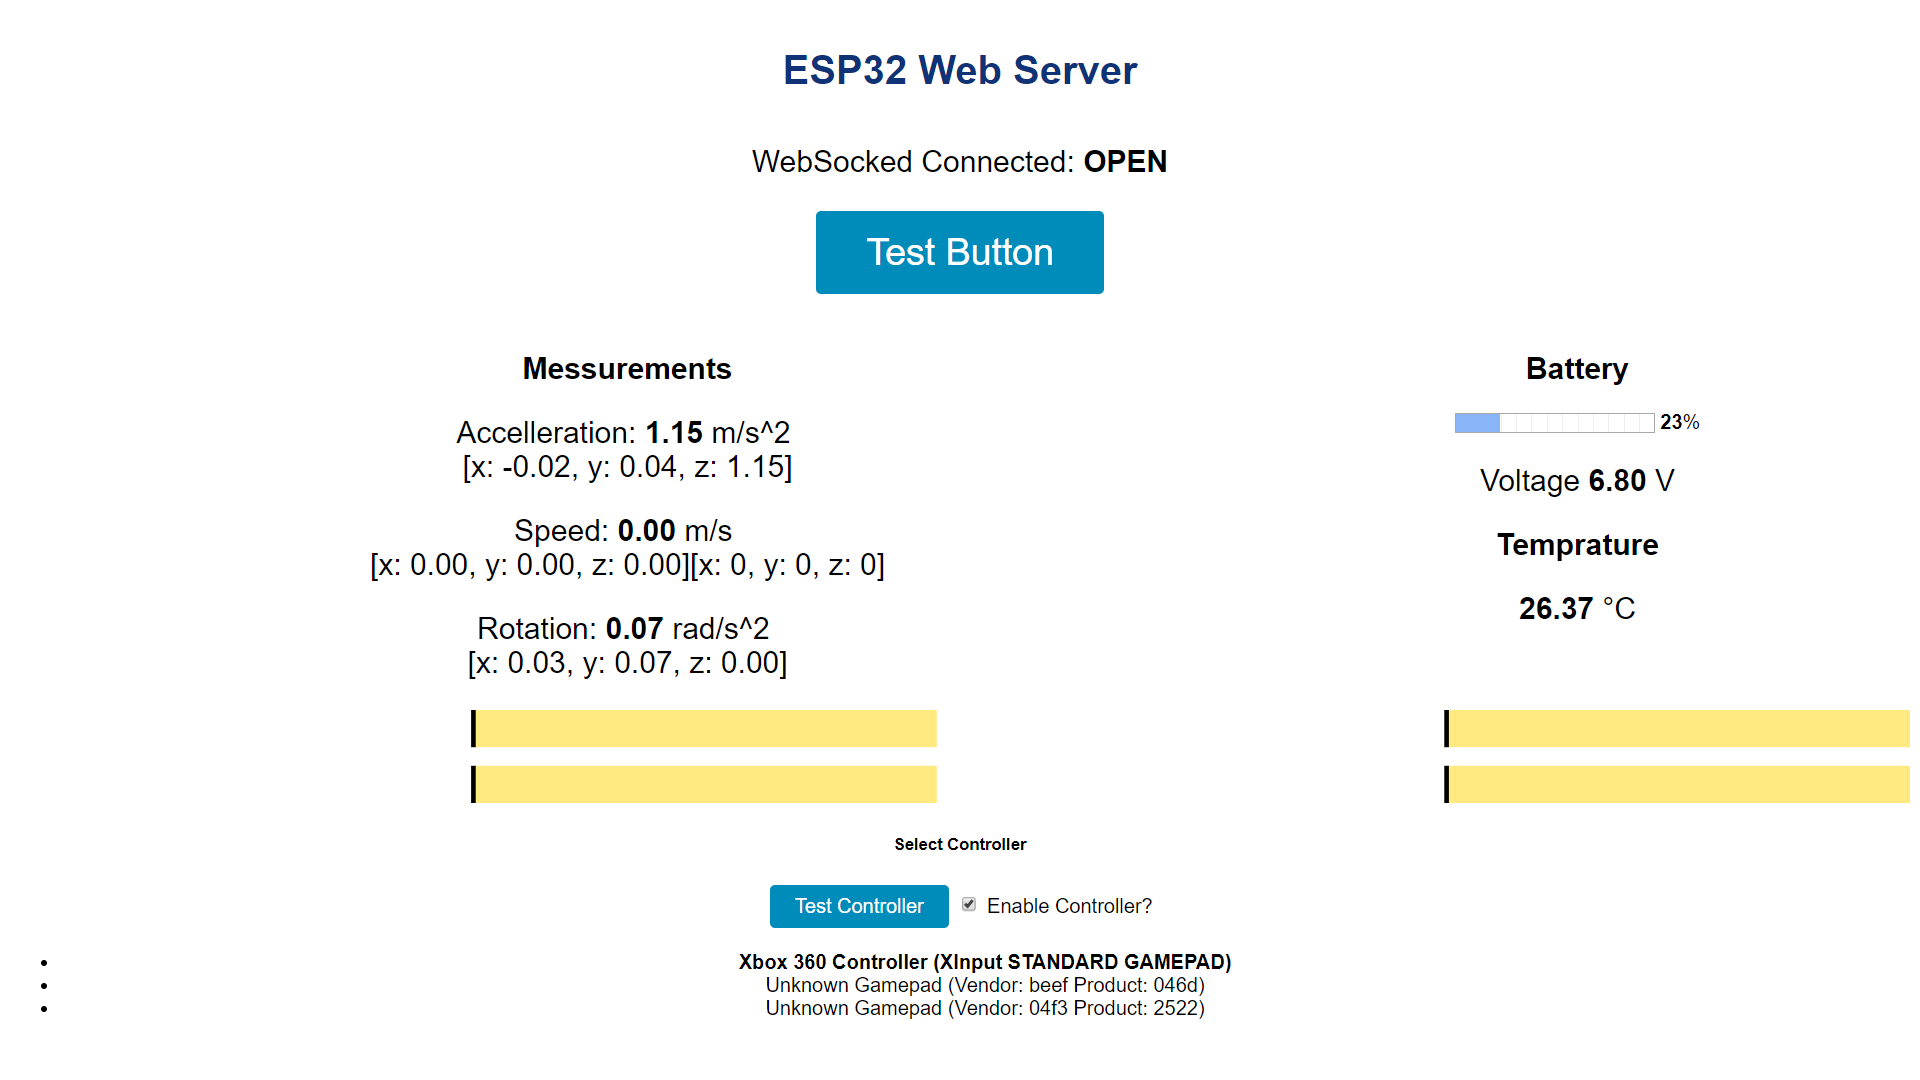
\includegraphics[width=\textwidth]{bilder/WebValues.png}
	\caption{Bildschirmfoto Weboberfläche}
	\label{bild:webvalues}
\end{figure}

In der Weboberfläche (Abb.~\ref{bild:webvalues}) sind ebenfalls noch jegliche Messwerte hinterlegt, die das Fahrzeug sammelt.\par

Diese sind:\par

\begin{itemize}
	\item Beschleunigung 
	\item Geschwindigkeit
	\item Rotationsgeschwindigkeit
	\item Batteriespannung
	\item Temperatur
	\item Drehgeschwindigkeit der jeweiligen Motoren
\end{itemize}\par


\vspace{\baselineskip}
Für die Wahl des Controllers ist eine auswählbare Liste aller angeschlossenen Controller am Ende der Seite vorhanden. Falls der Nutzer keinen Controller besitzt oder angeschlossen hat, kann durch das Abwählen der Checkbox auf die Steuerung per WASD, sowie die Pfeiltasten gewechselt werden.\par

\subsection{Protokoll}
Zum Übertragen wurde ein binäres Protokoll (Tabelle~\ref{table:protokoll}) entwickelt, um die Datenrate gering zu halten, sowie die Verarbeitung auf dem Microcontroller zu vereinfachen.\par

Da durch Websockets bereits ein Integrierter Frame geschickt wird, muss nicht bei jeder Nachricht die Länge und Anfangs- und Endbyte mitgeschickt werden, wie es sonst bei raw Sockets nötig gewesen wäre.\par

Hierbei wird jeder Wert als Int16 geschickt, um ein ausreichend großes Spektrum bei geringer Datenrate zu gewährleisten. \par

Am Anfang jeder Nachricht wird die ID ebenfalls als int16 geschickt, somit wären 65536 unterschiedliche Nachrichten erlaubt.\par

Um die Anzahl an Nachrichten zu verringern, wurden die Batteriespannung und Werte des Gyroskop zu einer kombinierte Nachricht zusammengefasst, um den Overhead gering zu halten.\par

\begin{table}[ht]
	\centering
	\resizebox{\textwidth}{!}{
\begin{tabular}{|c|c|c|c|c|c|c|c|c|c|c|c|c|}
	\hline 
	\textbf{Name} & \textbf{ID} & \multicolumn{11}{c|}{\textbf{Werte}} \\ 
	\hline 
	\hline 
	DRIVE & 0 & X-Achse L & Y-Achse L & X-Achse R & Y-Achse R &  &  &  &  &  &  &  \\ 
	\hline 
	GYRO & 1 & Speed-X & Speed-Y & Speed-Z & Accel-X & Accel-Y & Accel-Z & Rot-X & Rot-Y & Rot-Z  &  & \\ 
	\hline 
	BATTERY & 2 & Voltage &  &  &  &  &  &  &  &  &  &  \\ 
	\hline 
	MOTOR & 3 & Speed-M1 & Speed-M2 & Speed-M3 & Speed-M4 &  &  &  &  &  &  &  \\ 
	\hline 
	COMB & 4 & Speed-X & Speed-Y & Speed-Z & Accel-X & Accel-Y & Accel-Z & Rot-X & Rot-Y & Rot-Z  & Battery & Temp \\ 
	\hline 
\end{tabular}} 
\caption{Binäres Protokoll} 
\label{table:protokoll}
\end{table} 



\section{Steuerung per (XBox) Controller}
Wie bereits in der Dokumentation der Weboberfläche erwähnt, wird die Steuerung primär per Spiele Controller gelöst, beispielsweise einen XBox-Controller von Microsoft.
Diese Entscheidung ist in der erhöhten Mobilität motiviert. 

Mit einer Stuerung per WASD bzw. per Pfeiltasten sind nur binäre Zustände messbar, gedrückt oder nicht gedrückt, volle Geschwindigkeit oder Stillstand.
Im Vergleich dazu erlauben uns die JoySticks des Controllers durch unterschiedlich stare Auslenkung die Geschwindigkeit sehr variabel zu bestimmen.

Da hierbei ebenfalls der JoyStick in jegliche Richtungen bewegt werden kann, können ebenfalls die Mecanum Räder so angesteuert werden, dass sie in genau diese Richtung fahren.

Jedoch sind hiermit nur zwei der drei Freiheitsgrade unserer Fahrzeugs abgedeckt. Um Rotationen um die eigene Achse mit variabler Geschwindigkeit zu steuern, wird die Eingabe des linken und des rechten JoySticks mit folgenden Formelen überlagert.

\bigskip
Sei hier $controlSide$ Auslenkung des linken Sticks in X Richtung (nach rechts), 
$controlFront$ Auslenkung des linken Sticks in Y Richtung (nach vorne) und 
$controlTurn$ Auslenkung des rechten Sticks in X Richtung (nach rechts), 

\begin{align}
	\phi = atan2(controlSide, controlFront)\\
	vd = min(\sqrt{controlFront^2 + controlSide^2}, 1023) - \frac{controlTurn}{2}\\
	vphi = \frac{controlTurn}{2}
\end{align}


\section{PLA vs. TPU}

\section{Eierhalter}					

\section{Leichtbau}	